% Created by tikzDevice version 0.10.1 on 2018-01-23 16:20:11
% !TEX encoding = UTF-8 Unicode
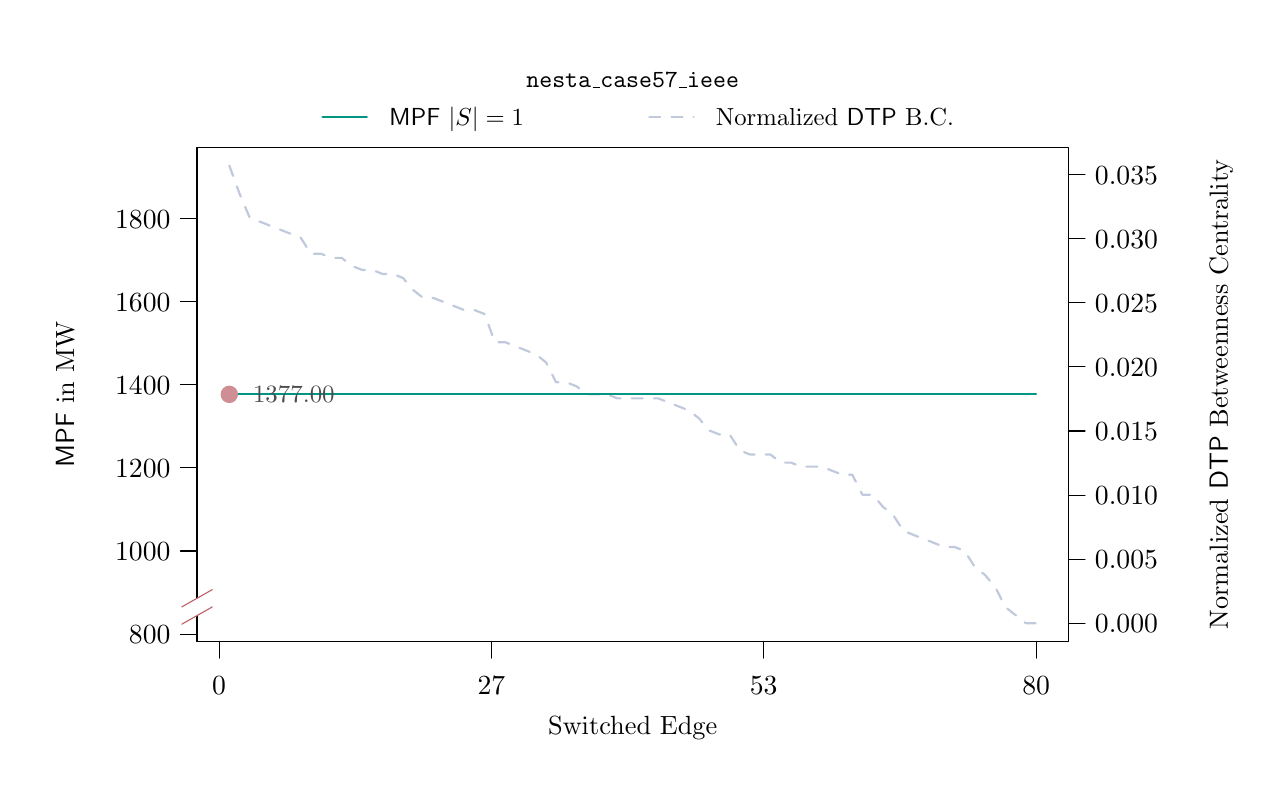
\begin{tikzpicture}[x=1pt,y=1pt]
\definecolor{fillColor}{RGB}{255,255,255}
\path[use as bounding box,fill=fillColor,fill opacity=0.00] (0,0) rectangle (440.85,271.01);
\begin{scope}
\path[clip] (  0.00,  0.00) rectangle (440.85,271.01);
\definecolor{drawColor}{RGB}{193,202,220}

\path[draw=drawColor,line width= 0.8pt,dash pattern=on 4pt off 4pt ,line join=round,line cap=round] ( 72.86,221.20) --
	( 76.55,211.04) --
	( 80.24,202.34) --
	( 83.93,200.89) --
	( 87.62,199.44) --
	( 91.31,197.99) --
	( 95.00,196.54) --
	( 98.69,195.08) --
	(102.38,189.28) --
	(106.07,189.28) --
	(109.76,187.83) --
	(113.45,187.83) --
	(117.14,184.93) --
	(120.83,183.48) --
	(124.52,183.48) --
	(128.21,182.03) --
	(131.90,182.03) --
	(135.59,180.58) --
	(139.28,176.22) --
	(142.97,173.32) --
	(146.66,173.32) --
	(150.35,171.87) --
	(154.05,170.42) --
	(157.74,168.97) --
	(161.43,168.97) --
	(165.12,167.52) --
	(168.81,157.37) --
	(172.50,157.37) --
	(176.19,155.91) --
	(179.88,154.46) --
	(183.57,153.01) --
	(187.26,150.11) --
	(190.95,142.86) --
	(194.64,142.86) --
	(198.33,141.41) --
	(202.02,138.51) --
	(205.71,138.51) --
	(209.40,138.51) --
	(213.09,137.06) --
	(216.78,137.06) --
	(220.47,137.06) --
	(224.16,137.06) --
	(227.85,137.06) --
	(231.54,135.60) --
	(235.23,134.15) --
	(238.92,132.70) --
	(242.61,129.80) --
	(246.30,125.45) --
	(249.99,124.00) --
	(253.68,124.00) --
	(257.37,118.20) --
	(261.06,116.75) --
	(264.75,116.75) --
	(268.44,116.75) --
	(272.13,113.84) --
	(275.82,113.84) --
	(279.51,112.39) --
	(283.20,112.39) --
	(286.89,112.39) --
	(290.58,110.94) --
	(294.27,109.49) --
	(297.96,109.49) --
	(301.65,102.24) --
	(305.34,102.24) --
	(309.03, 97.89) --
	(312.72, 94.98) --
	(316.41, 89.18) --
	(320.10, 87.73) --
	(323.79, 86.28) --
	(327.48, 84.83) --
	(331.17, 83.38) --
	(334.86, 83.38) --
	(338.55, 81.93) --
	(342.24, 76.13) --
	(345.94, 73.22) --
	(349.63, 68.87) --
	(353.32, 61.62) --
	(357.01, 58.72) --
	(360.70, 55.82) --
	(364.39, 55.82);
\end{scope}
\begin{scope}
\path[clip] (  0.00,  0.00) rectangle (440.85,271.01);
\definecolor{drawColor}{RGB}{0,0,0}

\path[draw=drawColor,line width= 0.4pt,line join=round,line cap=round] ( 61.20, 49.20) --
	(376.05, 49.20) --
	(376.05,227.81) --
	( 61.20,227.81) --
	( 61.20, 49.20);
\end{scope}
\begin{scope}
\path[clip] (  0.00,  0.00) rectangle (440.85,271.01);
\definecolor{drawColor}{RGB}{0,0,0}

\path[draw=drawColor,line width= 0.4pt,line join=round,line cap=round] (376.05, 55.82) -- (376.05,217.89);

\path[draw=drawColor,line width= 0.4pt,line join=round,line cap=round] (376.05, 55.82) -- (382.05, 55.82);

\path[draw=drawColor,line width= 0.4pt,line join=round,line cap=round] (376.05, 78.97) -- (382.05, 78.97);

\path[draw=drawColor,line width= 0.4pt,line join=round,line cap=round] (376.05,102.12) -- (382.05,102.12);

\path[draw=drawColor,line width= 0.4pt,line join=round,line cap=round] (376.05,125.28) -- (382.05,125.28);

\path[draw=drawColor,line width= 0.4pt,line join=round,line cap=round] (376.05,148.43) -- (382.05,148.43);

\path[draw=drawColor,line width= 0.4pt,line join=round,line cap=round] (376.05,171.58) -- (382.05,171.58);

\path[draw=drawColor,line width= 0.4pt,line join=round,line cap=round] (376.05,194.74) -- (382.05,194.74);

\path[draw=drawColor,line width= 0.4pt,line join=round,line cap=round] (376.05,217.89) -- (382.05,217.89);

\node[text=drawColor,anchor=base west,inner sep=0pt, outer sep=0pt, scale=  1.00] at (385.65, 52.37) {0.000};

\node[text=drawColor,anchor=base west,inner sep=0pt, outer sep=0pt, scale=  1.00] at (385.65, 75.53) {0.005};

\node[text=drawColor,anchor=base west,inner sep=0pt, outer sep=0pt, scale=  1.00] at (385.65, 98.68) {0.010};

\node[text=drawColor,anchor=base west,inner sep=0pt, outer sep=0pt, scale=  1.00] at (385.65,121.83) {0.015};

\node[text=drawColor,anchor=base west,inner sep=0pt, outer sep=0pt, scale=  1.00] at (385.65,144.99) {0.020};

\node[text=drawColor,anchor=base west,inner sep=0pt, outer sep=0pt, scale=  1.00] at (385.65,168.14) {0.025};

\node[text=drawColor,anchor=base west,inner sep=0pt, outer sep=0pt, scale=  1.00] at (385.65,191.29) {0.030};

\node[text=drawColor,anchor=base west,inner sep=0pt, outer sep=0pt, scale=  1.00] at (385.65,214.45) {0.035};
\end{scope}
\begin{scope}
\path[clip] (  0.00,  0.00) rectangle (440.85,271.01);
\definecolor{drawColor}{RGB}{0,150,130}

\path[draw=drawColor,line width= 0.8pt,line join=round,line cap=round] (106.55,238.60) -- (122.57,238.60);
\definecolor{drawColor}{RGB}{193,202,220}

\path[draw=drawColor,line width= 0.8pt,dash pattern=on 4pt off 4pt ,line join=round,line cap=round] (224.63,238.60) -- (240.65,238.60);
\definecolor{drawColor}{RGB}{0,0,0}

\node[text=drawColor,anchor=base,inner sep=0pt, outer sep=0pt, scale=  0.89] at (218.62,249.28) {\texttt{nesta\_case57\_ieee}};

\node[text=drawColor,anchor=base west,inner sep=0pt, outer sep=0pt, scale=  0.89] at (130.58,235.54) {$\mathsf{MPF}~|S|=1$};

\node[text=drawColor,anchor=base west,inner sep=0pt, outer sep=0pt, scale=  0.89] at (248.66,235.54) {Normalized~$\mathsf{DTP}$~B.C.};
\end{scope}
\begin{scope}
\path[clip] (  0.00,  0.00) rectangle (440.85,271.01);
\definecolor{drawColor}{RGB}{0,0,0}

\path[draw=drawColor,line width= 0.4pt,line join=round,line cap=round] ( 61.20, 51.88) -- ( 61.20,202.01);

\path[draw=drawColor,line width= 0.4pt,line join=round,line cap=round] ( 61.20, 51.88) -- ( 55.20, 51.88);

\path[draw=drawColor,line width= 0.4pt,line join=round,line cap=round] ( 61.20, 81.91) -- ( 55.20, 81.91);

\path[draw=drawColor,line width= 0.4pt,line join=round,line cap=round] ( 61.20,111.93) -- ( 55.20,111.93);

\path[draw=drawColor,line width= 0.4pt,line join=round,line cap=round] ( 61.20,141.96) -- ( 55.20,141.96);

\path[draw=drawColor,line width= 0.4pt,line join=round,line cap=round] ( 61.20,171.98) -- ( 55.20,171.98);

\path[draw=drawColor,line width= 0.4pt,line join=round,line cap=round] ( 61.20,202.01) -- ( 55.20,202.01);

\node[text=drawColor,anchor=base east,inner sep=0pt, outer sep=0pt, scale=  1.00] at ( 51.60, 48.44) {800};

\node[text=drawColor,anchor=base east,inner sep=0pt, outer sep=0pt, scale=  1.00] at ( 51.60, 78.46) {1000};

\node[text=drawColor,anchor=base east,inner sep=0pt, outer sep=0pt, scale=  1.00] at ( 51.60,108.49) {1200};

\node[text=drawColor,anchor=base east,inner sep=0pt, outer sep=0pt, scale=  1.00] at ( 51.60,138.52) {1400};

\node[text=drawColor,anchor=base east,inner sep=0pt, outer sep=0pt, scale=  1.00] at ( 51.60,168.54) {1600};

\node[text=drawColor,anchor=base east,inner sep=0pt, outer sep=0pt, scale=  1.00] at ( 51.60,198.57) {1800};
\end{scope}
\begin{scope}
\path[clip] (  0.00,  0.00) rectangle (440.85,271.01);
\definecolor{drawColor}{RGB}{255,255,255}
\definecolor{fillColor}{RGB}{255,255,255}

\path[draw=drawColor,line width= 0.4pt,line join=round,line cap=round,fill=fillColor] ( 55.69, 58.58) rectangle ( 66.71, 64.83);
\definecolor{drawColor}{RGB}{188,97,104}

\path[draw=drawColor,line width= 0.4pt,line join=round,line cap=round] ( 55.69, 55.45) -- ( 66.71, 61.70);

\path[draw=drawColor,line width= 0.4pt,line join=round,line cap=round] ( 55.69, 61.70) -- ( 66.71, 67.95);
\end{scope}
\begin{scope}
\path[clip] ( 61.20, 49.20) rectangle (376.05,227.81);
\definecolor{drawColor}{RGB}{0,150,130}

\path[draw=drawColor,line width= 0.8pt,line join=round,line cap=round] ( 72.86,138.51) --
	( 76.55,138.51) --
	( 80.24,138.51) --
	( 83.93,138.51) --
	( 87.62,138.51) --
	( 91.31,138.51) --
	( 95.00,138.51) --
	( 98.69,138.51) --
	(102.38,138.51) --
	(106.07,138.51) --
	(109.76,138.51) --
	(113.45,138.51) --
	(117.14,138.51) --
	(120.83,138.51) --
	(124.52,138.51) --
	(128.21,138.51) --
	(131.90,138.51) --
	(135.59,138.51) --
	(139.28,138.51) --
	(142.97,138.51) --
	(146.66,138.51) --
	(150.35,138.51) --
	(154.05,138.51) --
	(157.74,138.51) --
	(161.43,138.51) --
	(165.12,138.51) --
	(168.81,138.51) --
	(172.50,138.51) --
	(176.19,138.51) --
	(179.88,138.51) --
	(183.57,138.51) --
	(187.26,138.51) --
	(190.95,138.51) --
	(194.64,138.51) --
	(198.33,138.51) --
	(202.02,138.51) --
	(205.71,138.51) --
	(209.40,138.51) --
	(213.09,138.51) --
	(216.78,138.51) --
	(220.47,138.51) --
	(224.16,138.51) --
	(227.85,138.51) --
	(231.54,138.51) --
	(235.23,138.51) --
	(238.92,138.51) --
	(242.61,138.51) --
	(246.30,138.51) --
	(249.99,138.51) --
	(253.68,138.51) --
	(257.37,138.51) --
	(261.06,138.51) --
	(264.75,138.51) --
	(268.44,138.51) --
	(272.13,138.51) --
	(275.82,138.51) --
	(279.51,138.51) --
	(283.20,138.51) --
	(286.89,138.51) --
	(290.58,138.51) --
	(294.27,138.51) --
	(297.96,138.51) --
	(301.65,138.51) --
	(305.34,138.51) --
	(309.03,138.51) --
	(312.72,138.51) --
	(316.41,138.51) --
	(320.10,138.51) --
	(323.79,138.51) --
	(327.48,138.51) --
	(331.17,138.51) --
	(334.86,138.51) --
	(338.55,138.51) --
	(342.24,138.51) --
	(345.94,138.51) --
	(349.63,138.51) --
	(353.32,138.51) --
	(357.01,138.51) --
	(360.70,138.51) --
	(364.39,138.51);
\end{scope}
\begin{scope}
\path[clip] ( 61.20, 49.20) rectangle (376.05,227.81);
\definecolor{fillColor}{RGB}{207,142,147}

\path[fill=fillColor] ( 72.86,138.51) circle (  3.15);
\end{scope}
\begin{scope}
\path[clip] ( 61.20, 49.20) rectangle (376.05,227.81);
\definecolor{drawColor}{gray}{0.30}

\node[text=drawColor,anchor=base,inner sep=0pt, outer sep=0pt, scale=  0.90] at ( 96.18,135.62) {1377.00};
\end{scope}
\begin{scope}
\path[clip] (  0.00,  0.00) rectangle (440.85,271.01);
\definecolor{drawColor}{RGB}{0,0,0}

\path[draw=drawColor,line width= 0.4pt,line join=round,line cap=round] ( 69.17, 49.20) -- (364.39, 49.20);

\path[draw=drawColor,line width= 0.4pt,line join=round,line cap=round] ( 69.17, 49.20) -- ( 69.17, 43.20);

\path[draw=drawColor,line width= 0.4pt,line join=round,line cap=round] (167.58, 49.20) -- (167.58, 43.20);

\path[draw=drawColor,line width= 0.4pt,line join=round,line cap=round] (265.98, 49.20) -- (265.98, 43.20);

\path[draw=drawColor,line width= 0.4pt,line join=round,line cap=round] (364.39, 49.20) -- (364.39, 43.20);

\node[text=drawColor,anchor=base,inner sep=0pt, outer sep=0pt, scale=  1.00] at ( 69.17, 30.00) {0};

\node[text=drawColor,anchor=base,inner sep=0pt, outer sep=0pt, scale=  1.00] at (167.58, 30.00) {27};

\node[text=drawColor,anchor=base,inner sep=0pt, outer sep=0pt, scale=  1.00] at (265.98, 30.00) {53};

\node[text=drawColor,anchor=base,inner sep=0pt, outer sep=0pt, scale=  1.00] at (364.39, 30.00) {80};

\node[text=drawColor,anchor=base,inner sep=0pt, outer sep=0pt, scale=  0.95] at (218.62, 15.60) {Switched Edge};

\node[text=drawColor,rotate= 90.00,anchor=base,inner sep=0pt, outer sep=0pt, scale=  0.95] at ( 16.80,138.51) {$\mathsf{MPF}$ in~$\mathrm{MW}$};

\node[text=drawColor,rotate= 90.00,anchor=base,inner sep=0pt, outer sep=0pt, scale=  0.95] at (433.65,138.51) {Normalized~$\mathsf{DTP}$ Betweenness Centrality};
\end{scope}
\end{tikzpicture}
